\documentclass[11pt,ngerman]{article}
\usepackage[utf8]{inputenc}
%?
\usepackage[a4paper,left=2cm,right=2cm,top=2cm,bottom=2cm,bindingoffset=5mm]{geometry}
%?
\usepackage{hyperref}
\usepackage{booktabs}
\usepackage{graphicx}
\usepackage{enumitem}

\begin{document}
\title{Summary Computer Networks}
\author{John}
\maketitle

\setcounter{tocdepth}{1}
\tableofcontents
\newpage
\section{Motivation}

\subsection{Communication	Metaphors}
\begin{itemize}[noitemsep,nolistsep]
	\item Phase 1: Person to person
	\item Phase 2: Person to machine
	\item Phase 3: Machine to machine/Network of computers
	\item Phase 4: The internet of Things
\end{itemize}

\subsection{History}
\begin{itemize}[noitemsep,nolistsep]
	\item 1837:	Samuel	Morse	develops	the	telegraph
	\item 1953:	First	transatlantic	Telephone	line
	\item 1876:	Alexander	Graham	Bell	patents	the	telephone	(tele=distant,	phone=voice)
\end{itemize}

\subsection{Telephone	Network}
Existing	networks	are	going	to	be	integrated\\
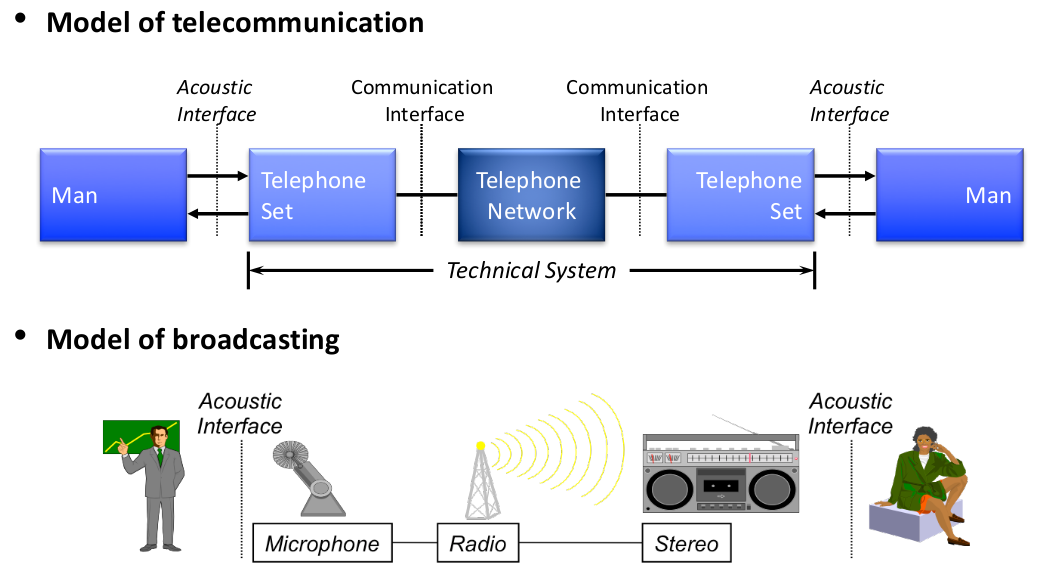
\includegraphics[width=5in]{images/Selection_001.png}

\subsection{The Internet}
The internet consists of
\begin{itemize}[noitemsep,nolistsep]
	\item a	set	of	computers,	which
	\begin{itemize}[noitemsep,nolistsep]
		\item use	the	TCP/IP	protocols
		\item are	somehow	(directly	or	indirectly)	connected
		\item offer	or	use	particular	services
	\end{itemize}
	\item a	set	of	users,	which	have	access	to	these	services
	\item a	set	of	other	networks,	which	(somehow)	are	accessible\\
\end{itemize}

\noindent Design Principles
\begin{itemize}[noitemsep,nolistsep]
	\item Minimalism	and	autonomy  - The	network	operates	by	itself	, does	not	require	internal	changes	when	new	networks	are	added
	\item Best-effort	service	model
	\item Soft-state	(stateless) - The	routers	do	not need	to	maintain end-to-end	communication	
information
	\item Decentralization
\end{itemize}



%%%%%%%%%%%%%%%%%%%%%%%%%%%%%%%%%%%%%%%%%%%%%%%%%%%%%%%%%%



\section{Introduction}
\subsection{Data	Communication}
Data	communication	is	the	processing	and	the	transport	of	digital	data	over	
connections	between	computers	(generally	over	large	distances).\\
Data	communication	comprises	two areas: Computer	Networks and Communication	Protocols

\subsection{What	is	Digital	Data?}
\begin{itemize}[noitemsep,nolistsep]
	\item Data: Representation	of	facts in	a	formal	way, processable by humans and machines, e.g. a language
	\item Information:  is	whatever	contributes	
to	a	reduction	in	the	uncertainty	of	the	state	of	a	system, can only be handled by humans
	\item Signal: is	the	physical	representation	
of	data	by	spatial	or	timely	variation	
of	physical	characteristics
	\item Example:  Sounds	of	a	language	(Data)	during	speaking	are	acoustic	waves	(Signals)
\end{itemize}

\subsection{Data	Communication}
\begin{itemize}[noitemsep,nolistsep]
	\item Sharing	resources	saves	costs
	\item Exchange	of	information
\end{itemize}

\subsection{Networking	Principles}
Communication	Peers
\begin{itemize}[noitemsep,nolistsep]
	\item Unicast:	Two	communication	peers	
communicate	over	a	Point-to-Point	
connection.
	\item Multicast:	One	sender	
communicates	to	several	receivers,	
which	are	known.
	\item Broadcast:	One	sender	transmits	to	
all	other	peers.
Typically	the	other	peers	are	
(partially)	unknown.
	\item Others:	Anycast,	Geocast,	etc.\\
\end{itemize}

\noindent Transmission
\begin{itemize}[noitemsep,nolistsep]
	\item Serial Transmission
	\item Parallel Transmission (Problem: synchronisation of the data)
	\item Asynchronous Transmission:	Transmission	in	which	each	block	
(character)	is	individually	synchronized\\
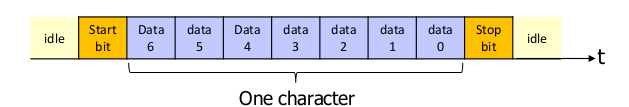
\includegraphics[width=5in]{images/Selection_002.png}

	\item Synchronous Transmission:	Transmission	in	which	the	time	of	
occurrence	of	each	signal	representing	a	bit	is	related	to	a	fixed	time	
frame \\
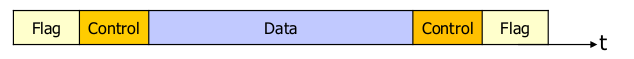
\includegraphics[width=5in]{images/Selection_003.png}
\end{itemize}

\noindent Connection	Properties
\begin{itemize}[noitemsep,nolistsep]
\item Simplex
\item Duplex
\item Half-Duplex\\
\end{itemize}

\noindent Multiplexing:
Combining	multiple	data	
channels	into	a	single	data	
channel	at	the	source\\

\noindent Quality\\
\begin{itemize}[noitemsep,nolistsep]
	\item Technical	Performance (Delay-Bandwidth-Product	=	
Store	capacity of	the	line)
	\begin{itemize}[noitemsep,nolistsep]
		\item Delay	[s]
		\item Jitter	[s]
		\item Throughput	[bit/s]
		\item Data	rate	[bit/s] (wird vorgegeben)
	\end{itemize}
	\item Costs
	\item Reliability
	\item Security	and	Protection\\
\end{itemize}

	\noindent	Safety measures: Encryption, Trustworthy	systems	\\
	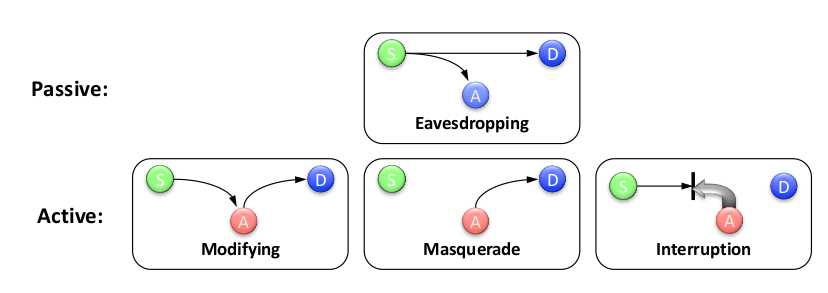
\includegraphics[width=5in]{images/Selection_005.png}


\noindent The	Client/Server	Principle
\begin{itemize}[noitemsep,nolistsep]
	\item Client $\rightarrow$ Server: Request
	\item Server $\rightarrow$ Client: Reply 
\end{itemize}
\begin{itemize}[noitemsep,nolistsep]
	\item Advantages
	\begin{itemize}[noitemsep,nolistsep]  
	\item Cost	reduction
	\item Better	usage	of	resources
	\item Modular	extensions
	\item Reliability	by	redundancy
	 \end{itemize}
	\item Server: Program	(process)	which	offers	a	service	over	a	network.	
	\item Client: Program	(process)	which	uses	a	service	offered	by	a	server.\\
\end{itemize}


\noindent Peer-to-Peer	Principle (ursprüngliche Kommunikation im Internet)
\begin{itemize}[noitemsep,nolistsep]
	\item Equal	partners,	no	fixed	client	and	server	roles
	\item Connections	between	any	pair	of	computers
	\item Establishment	of	a	whole	network	of	connections
	\item Best	example:	File	Sharing,	e.g.,	Napster,	Gnutella
\end{itemize}

\subsection{Communication	Protocols}

A	protocol	is	the	set	of	agreements	between	(application)	processes	with	the	purpose	of	
communication.\\
To	enable	understanding	in	communication,	all	communication	partners	have	to	speak	the	
same	language.
\begin{itemize}[noitemsep,nolistsep]
\item Data	formats	and	their	semantics
\item Control	over	media	access
\item Priorities
\item Handling	of	transmission	errors
\item Sequence	control
\item Flow	control	mechanisms
\item Segmentation	and	composition	of	long	messages
\item Multiplexing
\item Routing
\end{itemize}
	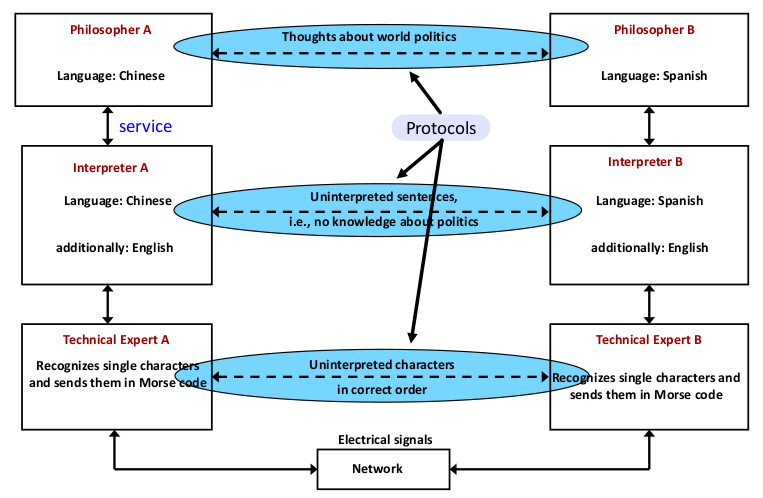
\includegraphics[width=5in]{images/Selection_006.png}\\
	$\rightarrow$ communication between horizontal layers
	
\noindent Peer	of	a	Layer
\begin{itemize}[noitemsep,nolistsep]
\item
use	one	service	
(except	the	bottom)
\item
offer	a	service	
(except	the	top)
\item
do	not	need	to	know	other	
than	the	next	lower	one
\item
talk	according	to	the	rules
\end{itemize}

\noindent Communication	architectures	are	based	on
\begin{itemize}[noitemsep,nolistsep]
\item  Service	=	Communication	Service
\item Rules	=	Communication	Protocol

\end{itemize}
A	service	is	offered	from	a	service	provider at	a	service	interface	
to	service	users.\\
Types	of	services	are:
\begin{itemize}[noitemsep,nolistsep]
\item Request
\item Indication
\item Response
\item Confirmation
\end{itemize}

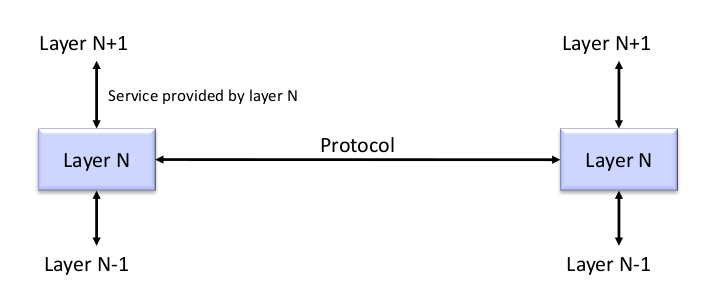
\includegraphics[width=5in]{images/Selection_007.png}\\

\textbf{Types of Services}
\begin{itemize}[noitemsep,nolistsep]
\item Unacknowledged	Service
\begin{itemize}[noitemsep,nolistsep]
\item Modeled	after	the	postal	service
\item Initiated	by	the	service	user
\end{itemize}
\item Acknowledged	Service (Transaction)
\item Connection-oriented	Service
\begin{itemize}[noitemsep,nolistsep]
\item Modeled	after	the	telephone	system
\item Before	the	instances	on	Layer-(N)	can	
exchange	data,	a	connection	on	
Layer-(N-1)	has	to	be	established
\item Negotiation	of	protocol	parameters\\
$\rightarrow$ Communication	context
\end{itemize}
\item Connectionless	Service
\begin{itemize}[noitemsep,nolistsep]
\item  Modeled	after	the	postal	service
\item No	establishment	of	connection	on	a	
lower	layer	required\\
$\rightarrow$ No	communication	context
\end{itemize}
\end{itemize}

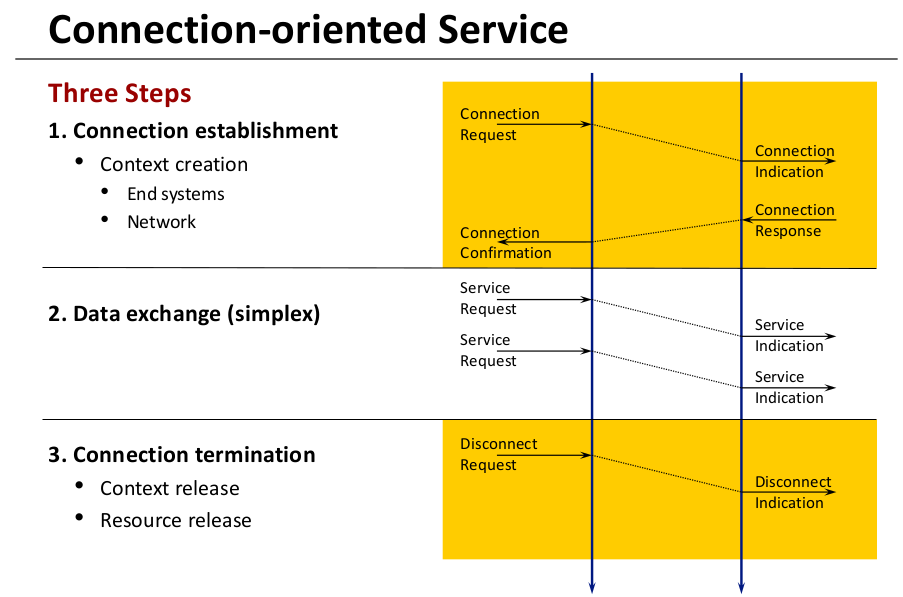
\includegraphics[width=5in]{images/Selection_008.png}\\
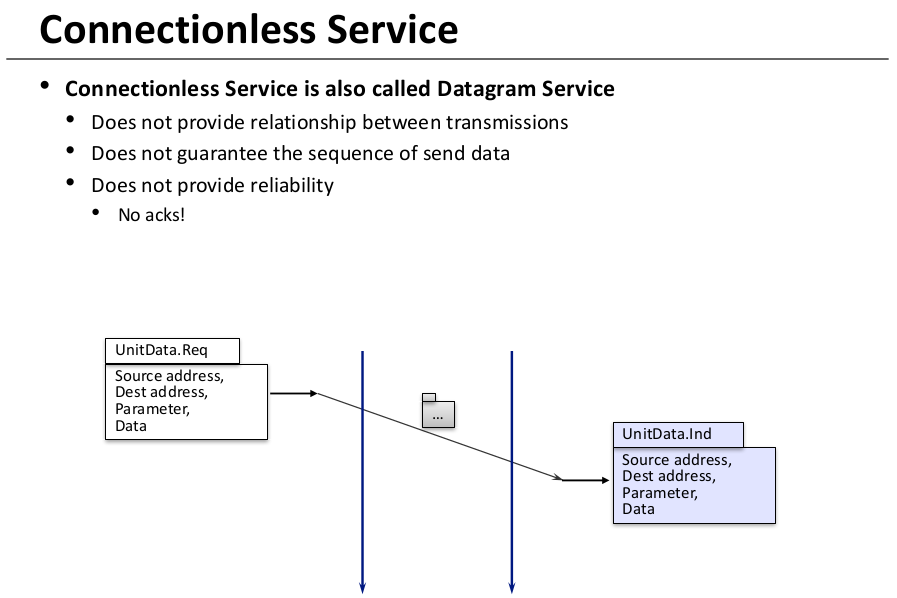
\includegraphics[width=5in]{images/Selection_009.png}\\

\textbf{Service primitives}\\
\begin{tabular}[t]{ll}
Primitive & Meaning\\
\hline
LISTEN & Block	waiting	for	an	incoming	connection\\
CONNECT & Establish	a	connection	with	a	waiting	peer\\
RECEIVE & Block	waiting	for	an	incoming	message\\
SEND & Send	a	message	to	the	peer\\
DISCONNECT & Terminate	a	connection\\
\end{tabular}\\
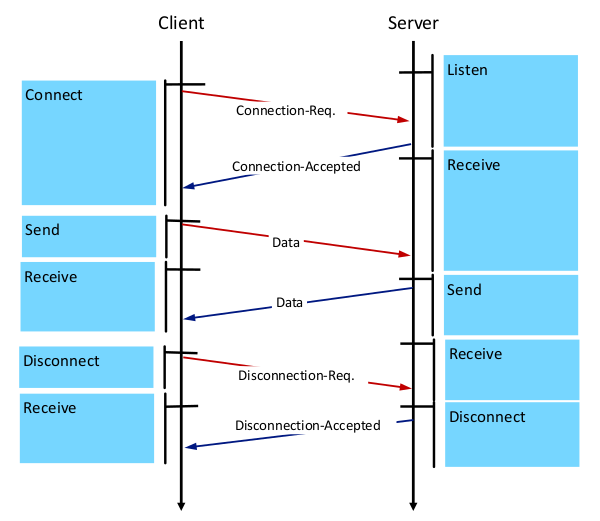
\includegraphics[width=3in]{images/Selection_010.png}\\

\subsection{ISO/OSI Reference Model}
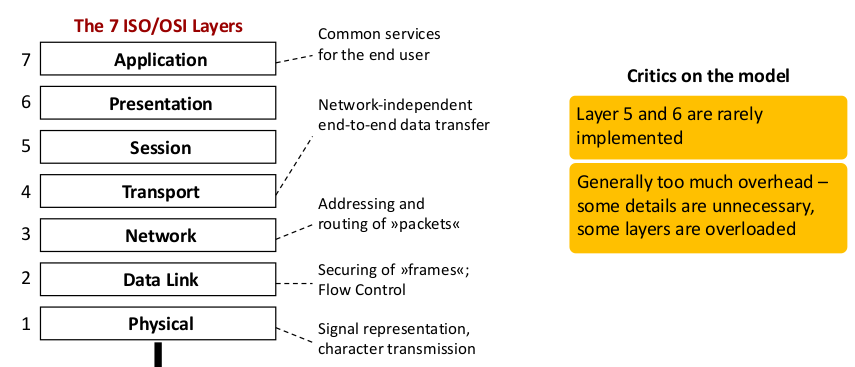
\includegraphics[width=5in]{images/Selection_011.png}\\

\begin{enumerate}[noitemsep,nolistsep]
\item Physical	Layer
	\begin{itemize}[noitemsep,nolistsep]
	\item Responsible for single bit transmission
	\item Details are defined: type	of	cables,	meaning	of	pins	of	network	
	connectors,	transmission	direction	on	the	cable
	\end{itemize}
	
\item Data Link Layer
	\begin{itemize}[noitemsep,nolistsep]
	\item Ensures	an	error-free data	transmission	between	two	directly	connected	
devices $\rightarrow$ segmented into frames (transmitted separately)
	\item Receiver checks the correctness (checksum)
	\item flow	control	is	used	to	control	the	re-transmission	of	corrupt	
frames	and	protect	the	receiver	from	overload.
	\item control	of	medium	access (prevent address conflict)
	\end{itemize}

\item Network Layer
	\begin{itemize}[noitemsep,nolistsep]
	\item Data-transmission over	large	distances	and	
between	heterogeneous	sub-networks
	\item uniform	addressing	of	hosts
	\item 	routing:	select	a	path	through	the	network.		
	\item Quality	of	Service	(QoS)	issues,	i.e.,	if	too	many	packets	are	present	at	the	
same	time	in	the	network,	they	may	form	bottlenecks. (congestion, maximum size	of	the	transferred	data	units	(MTU), delay,	jitter,	transit	time,	etc.)
	\end{itemize}
	
\item Transport Layer
	\begin{itemize}[noitemsep,nolistsep]
	\item end-to-end	communication between	two	processes
	\item Ensure	that	the	data	are	receipt	complete and	in	correct	order
	\item current	network	state	is	monitored	to	adapt	to	the	
receiver	and	to	the	network	capacity
	\end{itemize}
	
\item Session Layer
	\begin{itemize}[noitemsep,nolistsep]
	\item manages	reliable	data	transport
	\item offers dialogue	
control,	i.e.,	define	the	direction	of	the	transmission.
	\item token	management (allows operation)
	\item set synchronization	points in the communication process
	\end{itemize}
	
\item Presentation	Layer
	\begin{itemize}[noitemsep,nolistsep]
	\item Represent	the	data	to	be	transmitted	in	a	way,	that	they	can	be	handled	from	
different	computer	systems	
	\item Data	are	encoded in	an	abstract (and	commonly	recognized)	data	format	before	
the	transmission	and	are	coded	back	by	the	receiver	into	its	own	data	format.
	\end{itemize}
	
\item Application	Layer
	\begin{itemize}[noitemsep,nolistsep]
	\item standard protocols	are	provided,	that	can	be	used	from	
applications
	\item interface	to	file	transfer
	\end{itemize}
\end{enumerate}

\textbf{Interplay	between	the	Layers
}\begin{itemize}[noitemsep,nolistsep]
\item Layer	(N-1)	offers	its	functionality	to	layer	N	as	a	communication	service.
\item Layer N	enhances	the	data	to	be	sent	with	control	information	(Header)	and	sends	the	data	
together	with	the	header	as Protocol	Data	Units (PDU).
\item Depending on the protocol, N-PDUs can be segmented into several
(N-1)-PDUs before transmission
\end{itemize}

\subsection{The	TCP/IP	Reference	Model}
\begin{enumerate}
	\item Host-to-Network	Layer (1+2)
		\begin{itemize}[noitemsep,nolistsep]
		\item Not defined exactly
		\item host	
must	be	connected	to	the	network	via	a	protocol	in	a	way	that	it	is	able	to	send	
and	receive	IP	datagrams
		\end{itemize}
	\item Internet	Layer (3)
		\begin{itemize}[noitemsep,nolistsep]
		\item 	interworking	of	different	networks
		\item enables	communication	between	hosts	over	the	own	network	
borders (	transmission	is	connectionless)
		\item  Router takes over the forwarding
		\item Path can be dynamic
		\item In	contrast	to	ISO,	only	one	packet	format	is	defined,	together	with	a	
connectionless	protocol,	the	Internet	Protocol	(IP)
		\end{itemize}
	\item Transport	Layer (4)
		\begin{itemize}[noitemsep,nolistsep]
		\item covers	the	communication	between	the	end	systems
		\item TCP (Transmission	Control	Protocol)	is	a	reliable,	connection-oriented protocol	
for	the	transmission	of	a	byte	stream between	two	hosts.
		\item UDP (User	Datagram	Protocol)	is	an	unreliable and	connectionless	protocol	
(best	effort).
		\end{itemize}
	\item Application	Layer (7)
		\begin{itemize}[noitemsep,nolistsep]
		\item defines	common	communication	services (HTTP, FTP,..)
		\end{itemize}
\end{enumerate}

\subsection{OSI	vs.	TCP/IP}

\begin{enumerate}[noitemsep,nolistsep]
	\item Time -
The	TCP/IP	protocols	were	already	widely	used	before	OSI	had	finished	the	
standardization	activities.
	\item Freedom	from	obligation (defines what not how) $\rightarrow$ incompatibility	of	products
	\item Complicatedness
	\item 	Political	reasons (Europe)
	\item Hurriedly	product	implementation
\end{enumerate}



\subsection{Standardization}
Two	types	of	standards
\begin{itemize}[noitemsep,nolistsep]
\item De	facto	standards
\item De	jure	standards
\end{itemize}

\noindent Organisationen:
\begin{itemize}[noitemsep,nolistsep]
\item ISO
\item Internet	Engineering	Task	Force
\item Institute	of	Electrical	and	Electronic	Engineers	(IEEE)
\end{itemize}

\subsection{Evolution	of	Computer	Networks}
\begin{itemize}[noitemsep,nolistsep]
\item First generation: via mainframe in computer center
\item Connection via LAN, router $\rightarrow$ rest of the world
\item computer centers via router connected to backbone $\rightarrow$ rest of the world
\end{itemize}

\subsection{Classification	of	Computer	Networks}
\begin{itemize}[noitemsep,nolistsep]
\item Personal	Area	Network	(PAN) - 1m
\item Local	Area	Network	(LAN) - 10-100m
\item Metropolitan	Area	Network	(MAN) - 1-10km
\item Wide	Area	Network	(WAN) - 100-1000km
\item Internet - 10000km 
\end{itemize}


%%%%%%%%%%%%%%%%%%%%%%%%%%%%%%%%%%%%%%%%%%%%%%%%%%%%%%%%%%%%%%%%%%%%%%%%%%%%%%%%%%%%%

\section{Physical Layer}

\subsection{Theoretical	Basis	for	Data	Communication}
\begin{itemize}[noitemsep,nolistsep]
\item Spectrum of	a	signal	is	the	range	of	
frequencies	it	contains
\item The	absolute	bandwidth of	the	signal	
is	the	width	of	the	spectrum
\item Bandwith of a medium: Frequency	range	which	can	be	
transmitted	over	a	medium
\end{itemize}

Transmission	of	information	can	take	place	on	
\begin{itemize}[noitemsep,nolistsep]
\item Baseband (information	is	transmitted	over	the	medium	as	it	is)\\
	$\rightarrow$ discrete	(digital) signals
\item Broadband (The	information	is	transmitted	analogous by modulating onto a carrier signal)\\
	used in optical and radio networks\\
	$\rightarrow$ continuous	(analogous)	signals
\end{itemize}

Nyquist- und	Shannon-Theorem\\
max.	data	rate	=	$2 \cdot B \cdot log_2 (n)$ vs. $B \cdot log_2 (1+SNR)$

\subsection{Analog	Data	and	Digital	Signals}

Pulse	Code	Modulation	(PCM)	is	based	on	the	sampling	theorem	
by	Shannon	and	Raabe: If	a	signal	is	sampled	at	regular	intervals	of	time	and	at	a	rate	higher	than	twice	the	highest	
significant	signal	frequency,	then	the	samples	contain	all	the	information	of	the	original	
signal.

\subsection{Data	Encoding}
see exercise
\subsection{Transmission	Media}
see exercise
\subsection{The	Last	Mile	Problem}
connect	private	homes	to	
the	Internet	without	installing	many	new	cables $\rightarrow$ Use	existing	telephone	lines:	re-use	them	for	data	
traffic\\

Examples: Modem, ISDN, DSL\\

Modulation:
\begin{itemize}[noitemsep,nolistsep]
\item Amplitude Modulation
\item Frequency Modulation
\item Phase Modulation
\end{itemize}

\subsection{Multiplexing}
Sharing	of	an	expensive	resource,	e.g.,	transmit	multiple	connections	over	
the	same	line\\
Frequency	Division	Multiplexing, Time	Division	Multiplexing

\subsection{Digital	Subscriber	Line	(DSL)}
Combination	of	usual	phone	service	
(analog/ISDN)	and	data	service: 
simply	use	the	whole	spectrum	a	copper	
cable	can	transfer,	not	only	the	range	up	to	
3.4	kHz!


\section{Data Link Layer}

\begin{itemize}[noitemsep,nolistsep]
\item provides	a	well-defined	service	
interface	to	the	network	layer
\item deals	with	transmission	errors
regulates
the	flow	of	data, 
the	access	to	the	medium, 
that	a	slow	receiver	is	not	swamped	by	
a	fast	sender
\end{itemize}

\noindent Parts:
\begin{itemize}[noitemsep,nolistsep]
\item Logical	Link	Control	(LLC)
\begin{itemize}[noitemsep,nolistsep]
\item  Organization	of	the	data	to	be	sent	into	frames
\item Guarantee	(if	possible)	an	error	free	transmission	between	neighboring nodes	by	...
\item Detection	(and	recovery)	of	transfer	errors
\item Flow	Control	(avoidance	of	overloading	the	receiver)
\item Buffer	Management
\end{itemize}
\item Medium	Access	Control	(MAC)
\begin{itemize}[noitemsep,nolistsep]
\item Access	control	to	the	communication	channel	in	broadcast	networks
\end{itemize}
\end{itemize}

\subsection{Error	Detection	and	Correction}
Compute	a	short	checksum	of	the	data	and	send	it	together	with	
the	data	to	the	receiver.	

CRC, Hamming Code $\rightarrow$ exercise

\subsection{Elementary	Data	Link	Protocols}

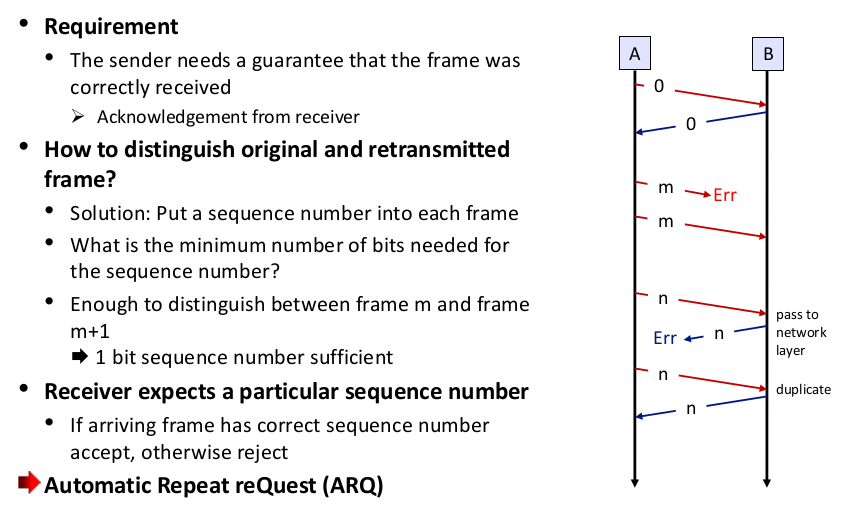
\includegraphics[width=5in]{images/Selection_016.png}

\textbf{Sliding Window}: Allow	sender	to	transmit	up	to	W
frames	before	blocking\\
 $\rightarrow$ exercise\\
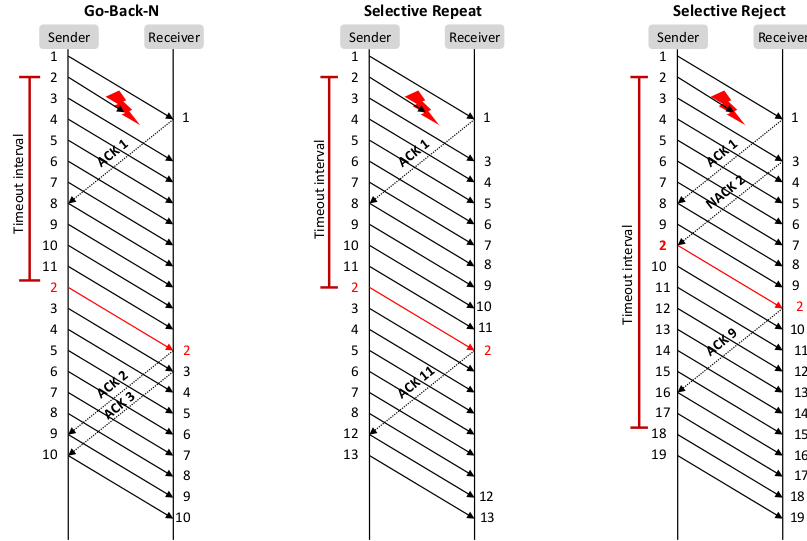
\includegraphics[width=5in]{images/Selection_017.png}

\subsection{High	Level	Data	Link	Control	(HDLC)}
Three	types	of	stations
\begin{itemize}[noitemsep,nolistsep]
\item Primary	station:	responsible	for	controlling	the	operation	of	the	link.	
\item Secondary	station:	operates	under	the	control	of	the	primary	station.	
\item Combined	station
\end{itemize}

\noindent \textbf{Bit stuffing:} Sender	inserts	a	zero	after	each	sequence	of	five	ones.	The	receiver	removes	this	
zero.\\
frame: 01111110 Address Control Data Checksum 01111110 \\
Control: 0 Seq P/F Next

\subsection{Point-to-Point	Protocol	(PPP)}
Establish	a	direct	connection	between	two	nodes\\
Features:
\begin{itemize}[noitemsep,nolistsep]
\item Framing	method	with	error	detection
\item Link	Control	Protocol
\item is	character	oriented	and	uses	byte-stuffing
\end{itemize}

\subsection{Protocol Verification}
\begin{itemize}[noitemsep,nolistsep]
\item Finite	state	machines
\item Petry nets
\end{itemize}

\section{Medium	Access	Control	Sublayer}
Two	kinds	of	connections	in	networks
\begin{itemize}[noitemsep,nolistsep]
\item Point-to-point	connections
\item Broadcast	
(Multi-access	channel,	Random	access	
channel)
\end{itemize}

In	a	network	with	broadcast	
connections $\rightarrow$ Who	gets	the	channel?

\subsection{The	Channel	Allocation	Problem}
Static	Channel	Allocation
\begin{itemize}[noitemsep,nolistsep]
\item Time	Division	Multiple	Access	(TDMA)
\item Frequency	Division	Multiple	Access	(FDMA)
\end{itemize}
$\rightarrow$ works only for fixed number of users, data traffic is bursty

\subsection{Multiple	Access	Protocols}
\textbf{ALOHA}	
\begin{itemize}[noitemsep,nolistsep]
\item Stations	are	sending	completely	uncoordinated	(random)
\item All	stations	use	the	same	frequency
\item When	two	(or	more)	stations	are	sending	at	the	same	time,	a	collision	occurs:	all	
messages	are	destroyed.	
\item repeat	after	a	random	time
\item Improvement:	Slotted	ALOHA $\rightarrow$ The	time	axis	is	divided	into	time	slots\\
\end{itemize}

\noindent \textbf{Carrier	Sense	Multiple	Access	(CSMA)}
\begin{itemize}[noitemsep,nolistsep]
\item 	each	station,	which	wants	to	send,	first	examines	whether	already	
another	station	is	sending
\item p-persistent	CSMA :  If	channel	idle,	station	transmits	with	probability	p in	current	slot	and	with	probability		(1-p)	it	defers	until	next	slot.
\item CSMA	with	Collision	Detection:	CSMA/CD
	\begin{itemize}[noitemsep,nolistsep]
	\item Basis	of	Ethernet
	\item A	station	who	detects	a	collision	stops	immediately	transmitting
	\item Afterwards	it	waits	a	random	time	and	tries	again
	\end{itemize}
\end{itemize}

\subsection{Multiple	Access	Protocols - Collision-Free	Protocols}
Split into reservation phase and transmission phase.

\begin{itemize}[noitemsep,nolistsep]
\item Bit-Map	Protocol 
	\begin{itemize}[noitemsep,nolistsep]
	\item without connection: set k-th bit in reservation frame
	\item with connection: try to write your station number in one contention slot
	\end{itemize}
\item Binary	Countdown: Compare addresses, 1 wins
\end{itemize}

\subsection{Multiple	Access	Protocols - Limited	Contention	Protocols}
\begin{itemize}[noitemsep,nolistsep]
\item Adaptive	Tree	Walk	Protocol
\item Coordination	by	using	a	Token
\end{itemize}

\subsection{Multiple	Access	Protocols - MAC	for	Wireless	Networks}
Multiple	Access	with	Collision	Avoidance	(MACA)
\begin{itemize}[noitemsep,nolistsep]
\item Idea:	Inform	stations	in	the	neighborhood	about	the	transmission
\item Ready	To	Send	(RTS)
\item Clear	To	Send	(CTS)
\item Extension	of	MACA	by	an	acknowledgement $\rightarrow$ MACAW
\end{itemize} 

\subsection{Ethernet}
Resolving	Collisions	in	Ethernet: Binary	Exponential	Backoff

\subsection{Network	Infrastructure}
\begin{itemize}[noitemsep,nolistsep]
\item Transparent	Bridges:	Address	Learning
\item Preventing	loops:	compute	a	
spanning	tree	from	all	connected	
bridges
\end{itemize}


\subsection{Virtual	LANs}
Decoupling	of	the	logical	topology from	the	physical	topology

\subsection{Summary}
Layer	1	defines	transmission	medium	and	bit	representation	on	this	medium, 
transmission	mode,	data	rate,	pin	usage	of	connectors,	...\\
Layer	2	protects	against	transmissions	errors	(mostly	CRC)	and	
receiver	overload	(flow	control,	sliding	window)\\
Layer	2	also	defines	medium	access	coordination	for	broadcast	networks\\
Both	layers	together	define	how	to	transfer	data	from	one	computer	to	a	
directly	connected	one,	thus	both	are	implemented	in	one	piece	of	
software:	the	network	interface	card	driver.

\section{Network	Layer}
\begin{itemize}[noitemsep,nolistsep]
\item Boundary	between	network	carrier	
and	customer
\item Control	of	global	traffic
\begin{itemize}[noitemsep,nolistsep]
	\item Coupling	of	sub-networks
	\item Global	addressing
	\item Routing	of	data	packets
	\item Initiation,	management,	and	 termination	of	connections	through	 the	whole	network
	\item Global	flow	control\\
\end{itemize}

\end{itemize}
\noindent Routers	in	the	network	receive frames from	layer	2,	
extract	the	layer	3	content	(packet)	and	decide	
based	on	the	global	address to	which	outgoing	
connection	(port)	the	packet	has	to	be	passed	on.	
Accordingly	the	packet	becomes	payload of	a	new	
frame	and	is	sent.

\subsection{Routing	principles}
\begin{itemize}[noitemsep,nolistsep]
	\item Connectionless	communication	(e.g.	Internet, packets	can	take	different	ways)
	\item Connection-Oriented	Communication 	(e.g.	telephony, virtual connection)\\
\end{itemize}

\noindent Routing: determine	most	favorable	route	from	the	source	node	to	the	
destination	node\\
Routing tables: can be determined statically or dynamically, can be one-, two- or multidimensional (optimization goals)

\subsection{Internet}
Goal:Interconnection	of	computers	and	networks	using	uniform	protocols
\begin{itemize}[noitemsep,nolistsep]
	\item ARPANET 	(predecessor	of	today's	Internet)
	\item All networks had different protocols $\rightarrow$ 	TCP/IP	networks
\end{itemize}
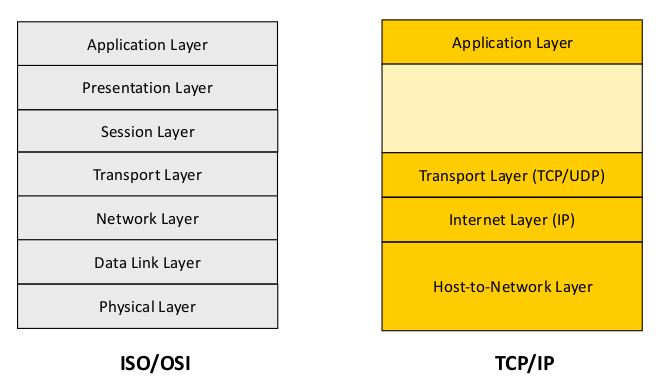
\includegraphics[width=5in]{images/Selection_018.png}

\subsection{Internet	Protocol	(IP)}
Raw	division	into	three	tasks
\begin{itemize}[noitemsep,nolistsep]
\item Data	transfer	over	a	global	network
\item Route	decision	at	the	sub-nodes
\item Control	of	the	network	or	transmission	status\\
\end{itemize}
connectionless,	unreliable	transmission	of	
datagrams/packets	$\rightarrow$ Best	Effort Service\\

\noindent \textbf{Subnets:} Some	bits	of	the	host	address	are	used	as	network	ID, 
A	Subnet	Mask	identifies	the	“abused”	bits\\
\textbf{Classless	Inter-Domain	Routing	(CIDR)}: Form	of	an	IP	address:	a.b.c.d/x  (The	first	x	bits	are	the	network	identification)

\subsection{IPv6}
\begin{itemize}[noitemsep,nolistsep]
\item Simpler structure of the headers
\item More automatism
\item Simpler configuration
\item Performance improvements
\item Migration strategies
\item More security
\item Larger address space (128 bit)
\item Flow	label: virtual	connection	with	certain	
characteristics/requirements
\end{itemize}

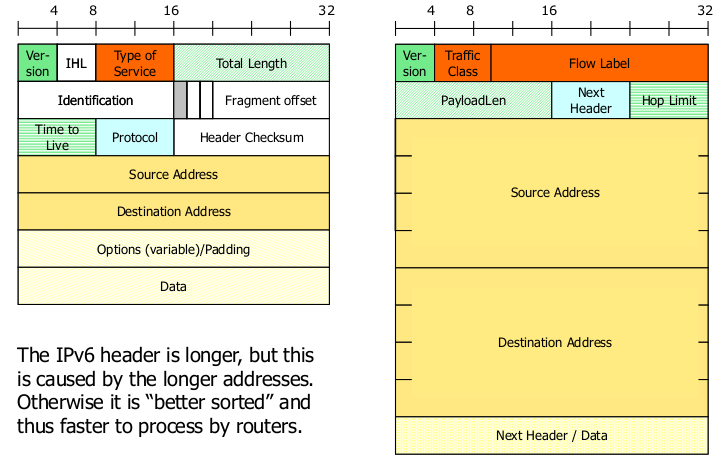
\includegraphics[width=6in]{images/Selection_019.png}

\noindent Three types of addresses:
\begin{itemize}[noitemsep,nolistsep]
\item Unicast
\item Anycast
\item Multicast (no broadcast)\\
\end{itemize}

Coexistence: 
\begin{itemize}[noitemsep,nolistsep]
\item Header Conversion ( Router	translates	an	incoming	IPv6	packet	into	a	IPv4	
packet,	receiving	router	retranslates)
\item  Tunneling  (encapsulates	an	incoming	IPv6	packet	into	
a	new	IPv4	packet)
\end{itemize}

\subsection{Network	Address	Translation}

\begin{itemize}[noitemsep,nolistsep]
\item Private address blocks  (10.0.0.0, 172.16.0.0, 192.168.0.0)
\item Router attached to the external world also need a global address
\item Basic	NAT	(also:	Static	NAT)
	\begin{itemize}[noitemsep,nolistsep]
	\item Each	private	IP	address	is	translated	into	one	certain	external	IP	address
	\item disadvantage: need as many official IP addresses as you have computers
	\end{itemize}
\item Hiding	NAT
	\begin{itemize}[noitemsep,nolistsep]
	\item Translates	several	local	addresses	into	the	same	external	address
	\item uses different ports
	\end{itemize}
\end{itemize}

\subsection{Auxiliary	Protocols}
\begin{itemize}[noitemsep,nolistsep]
\item Address	Resolution	Protocol	(ARP)
	\begin{itemize}[noitemsep,nolistsep]
	\item With	ARP,	IP	is	mapped	to	the	hardware	address	and	vice	versa
	\item ARP Request $\rightarrow$ ARP Response
	\end{itemize}
\item Reverse	Address	Resolution	Protocol	(RARP)
	\begin{itemize}[noitemsep,nolistsep]
	\item makes	it	possible	that	a	booted	machine	broadcasts	its	
hardware	address	and	gets	back	by	a	RARP	server	the	appropriate	IP	
address.	
	\item But: RARP-server in each local network required
	\end{itemize}
\item Dynamic	Host	Configuration	Protocol	(DHCP)
	\begin{itemize}[noitemsep,nolistsep]
	\item A computer	sends	a	DHCP	DISCOVER	packet.	In	each	subnet	a	
DHCP	Relay	Agent	is	placed,	who	passes	such	a	message	on	to	the	DHCP	
server.
	\end{itemize}
\item Internet	Control	Message	Protocol	(ICMP)
	\begin{itemize}[noitemsep,nolistsep]
	\item control	protocol	of	layer	3 if something unexpected happens (e.g.TTL=0)
	\item 	transmits	error	and	control	messages in an IP packet
	\end{itemize}
\item Internet	Group	Management	Protocol	(IGMP)
\end{itemize}

\section{Network Layer}
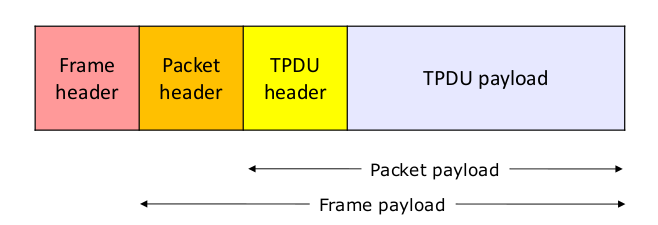
\includegraphics[width=5in]{images/Selection_020.png}\\
Messages	from	transport	entities:	
Transport	Protocol	Data	Unit	(TPDU)

\subsection{User	Datagram	Protocol	(UDP)}
\begin{itemize}[noitemsep,nolistsep]
	\item Like	IP:	Connectionless	and	unreliable
	\item No	acknowledgement
	\item Use	in	multicast
	\item Not reliable but fast
	\item Addressing	of	the	applications	by	\textbf{port numbers}
\end{itemize}

\subsection{Transport	Control	Protocol	(TCP)}
\begin{itemize}[noitemsep,nolistsep]
	\item Connection-oriented	and	reliable	(error-free,	keeps	packet	order,	without	duplicates)
	\item Byte	stream,	not	message	stream
	\item Error	handling,	acknowledgements,	flow	control	
	\item Urgent messages
	\item Addressing	of	the	application	by	port	numbers
	\item Establishes	logical	connections	between	two	\textbf{Sockets}
	\item TPDUs	are	called	segments
	\item Send	and 	receive	buffers\\
\end{itemize}

Ports:
\begin{itemize}[noitemsep,nolistsep]
\item 0-1023	System
\item 1024-49151 User
\item 49152-65535 Private
\end{itemize}

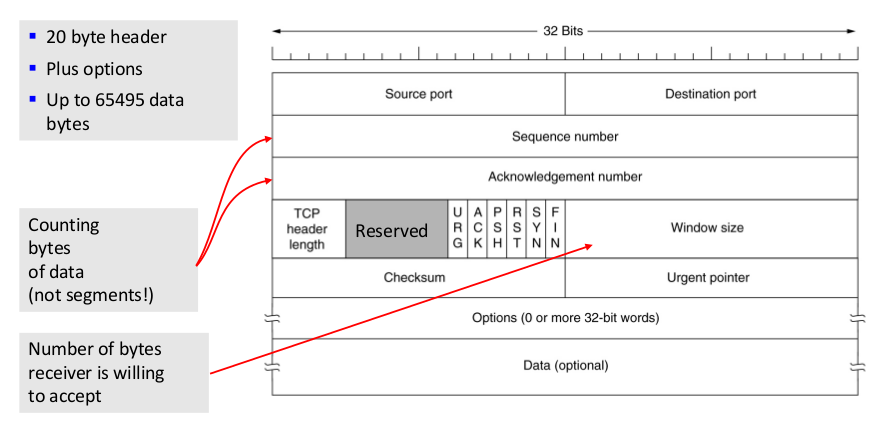
\includegraphics[width=6in]{images/Selection_021.png}\\

TCP	Connection	Management:	
\begin{enumerate}[noitemsep,nolistsep]
\item SYN, Seq=x
\item SYN, Seq=y, ACK=x+1
\item Seq=x+1, ACK=y+1
\end{enumerate}
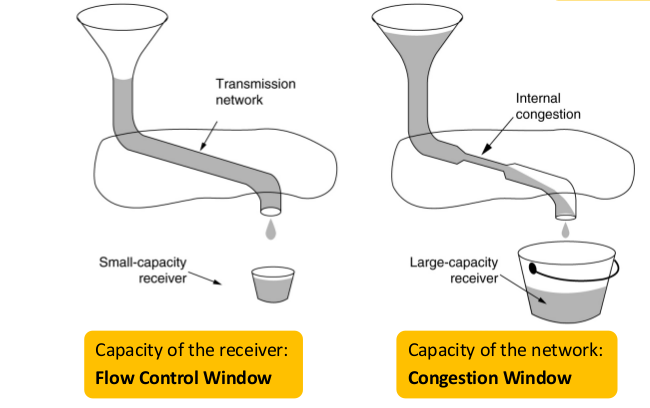
\includegraphics[width=5in]{images/Selection_022.png}\\



\end{document}